% Options for packages loaded elsewhere
\PassOptionsToPackage{unicode}{hyperref}
\PassOptionsToPackage{hyphens}{url}
\PassOptionsToPackage{dvipsnames,svgnames*,x11names*}{xcolor}
%
\documentclass[
]{article}
\usepackage{amsmath,amssymb}
\usepackage{lmodern}
\usepackage{ifxetex,ifluatex}
\ifnum 0\ifxetex 1\fi\ifluatex 1\fi=0 % if pdftex
  \usepackage[T1]{fontenc}
  \usepackage[utf8]{inputenc}
  \usepackage{textcomp} % provide euro and other symbols
\else % if luatex or xetex
  \usepackage{unicode-math}
  \defaultfontfeatures{Scale=MatchLowercase}
  \defaultfontfeatures[\rmfamily]{Ligatures=TeX,Scale=1}
\fi
% Use upquote if available, for straight quotes in verbatim environments
\IfFileExists{upquote.sty}{\usepackage{upquote}}{}
\IfFileExists{microtype.sty}{% use microtype if available
  \usepackage[]{microtype}
  \UseMicrotypeSet[protrusion]{basicmath} % disable protrusion for tt fonts
}{}
\makeatletter
\@ifundefined{KOMAClassName}{% if non-KOMA class
  \IfFileExists{parskip.sty}{%
    \usepackage{parskip}
  }{% else
    \setlength{\parindent}{0pt}
    \setlength{\parskip}{6pt plus 2pt minus 1pt}}
}{% if KOMA class
  \KOMAoptions{parskip=half}}
\makeatother
\usepackage{xcolor}
\IfFileExists{xurl.sty}{\usepackage{xurl}}{} % add URL line breaks if available
\IfFileExists{bookmark.sty}{\usepackage{bookmark}}{\usepackage{hyperref}}
\hypersetup{
  pdftitle={Meeting1},
  pdfauthor={Kuan Liu},
  colorlinks=true,
  linkcolor=Maroon,
  filecolor=Maroon,
  citecolor=Blue,
  urlcolor=blue,
  pdfcreator={LaTeX via pandoc}}
\urlstyle{same} % disable monospaced font for URLs
\usepackage[margin=1in]{geometry}
\usepackage{graphicx}
\makeatletter
\def\maxwidth{\ifdim\Gin@nat@width>\linewidth\linewidth\else\Gin@nat@width\fi}
\def\maxheight{\ifdim\Gin@nat@height>\textheight\textheight\else\Gin@nat@height\fi}
\makeatother
% Scale images if necessary, so that they will not overflow the page
% margins by default, and it is still possible to overwrite the defaults
% using explicit options in \includegraphics[width, height, ...]{}
\setkeys{Gin}{width=\maxwidth,height=\maxheight,keepaspectratio}
% Set default figure placement to htbp
\makeatletter
\def\fps@figure{htbp}
\makeatother
\setlength{\emergencystretch}{3em} % prevent overfull lines
\providecommand{\tightlist}{%
  \setlength{\itemsep}{0pt}\setlength{\parskip}{0pt}}
\setcounter{secnumdepth}{5}
\ifluatex
  \usepackage{selnolig}  % disable illegal ligatures
\fi

\title{Meeting1}
\author{Kuan Liu}
\date{Jul 20 2021}

\begin{document}
\maketitle

\hypertarget{chapter-1-statistical-approaches-for-clinicla-trials}{%
\section{Chapter 1 Statistical approaches for clinicla
trials}\label{chapter-1-statistical-approaches-for-clinicla-trials}}

\hypertarget{bayesian-versus-frequentist-appraoches-in-clincial-research}{%
\subsection{Bayesian versus frequentist appraoches in clincial
research}\label{bayesian-versus-frequentist-appraoches-in-clincial-research}}

\begin{itemize}
\tightlist
\item
  Key differences

  \begin{itemize}
  \tightlist
  \item
    parameters
  \item
    inference input data and prior
  \item
    \textbf{flexibility}, sequential learning
  \item
    probability statements, predictive probabilities
  \item
    decision theoretic
  \item
    comment on role of randomization
  \end{itemize}
\end{itemize}

Additional reading -
\href{http://www.stat.columbia.edu/~gelman/research/published/gelman_hennig_full_discussion.pdf}{Beyond
subjective and objective in statistics by Andrew Gelman and Christian
Henning} - Bayesian is no more subjective than frequentist - Prior can
be used meaningfully both computationally and biologically

\hypertarget{adaptivity}{%
\subsection{Adaptivity}\label{adaptivity}}

Bayesian is more commonly used for Phase I and Phase II trials. Some
appealing adoption including non-fixed sample-size, early stopping and
adoptive randomization.

\hypertarget{the-book-argue-full-bayesian-with-utility-function-is-awkward.}{%
\subsubsection{The book argue ``full bayesian'' with utility function is
awkward.}\label{the-book-argue-full-bayesian-with-utility-function-is-awkward.}}

\begin{itemize}
\tightlist
\item
  the expected utility function given poster distribution of the
  parameter
\item
  an example utility gain (or loss): Y(Z=1, treated)-Y(Z=0, control)
\end{itemize}

\[ \int u(\theta, x) p(\theta |x)d\theta \]

\hypertarget{bayes-as-a-frequentist-tool}{%
\subsubsection{Bayes as a frequentist
tool}\label{bayes-as-a-frequentist-tool}}

\begin{itemize}
\tightlist
\item
  flexibility, sequential learning
\item
  posterior predictive probability
\item
  use of prior, borrow info from other studies
\item
  adaptive randomization
\item
  seamless phase II and III design
\end{itemize}

\hypertarget{chapter-2-basics-of-bayesian}{%
\section{Chapter 2 Basics of
Bayesian}\label{chapter-2-basics-of-bayesian}}

Additional reading on choice of prior -
\url{https://github.com/stan-dev/stan/wiki/Prior-Choice-Recommendations}
-
\url{http://www.stat.columbia.edu/~gelman/research/unpublished/prior_context_2.pdf}

Additional reading on model selection (AIC, DIC, WAIC etc): -
\href{http://www.stat.columbia.edu/~gelman/research/published/waic_understand3.pdf}{Understanding
predictive information criteria for Bayesian models, Gelman, Hwang \&
Vehtari}

\hypertarget{principles-of-bayesian-clincial-trial-design}{%
\subsection{Principles of Bayesian clincial trial
design}\label{principles-of-bayesian-clincial-trial-design}}

Methods which can be used for clinical decision making

\begin{enumerate}
\def\labelenumi{\arabic{enumi}.}
\tightlist
\item
  Posterior predictive methods
\item
  Bayesian indifference zone methods
\end{enumerate}

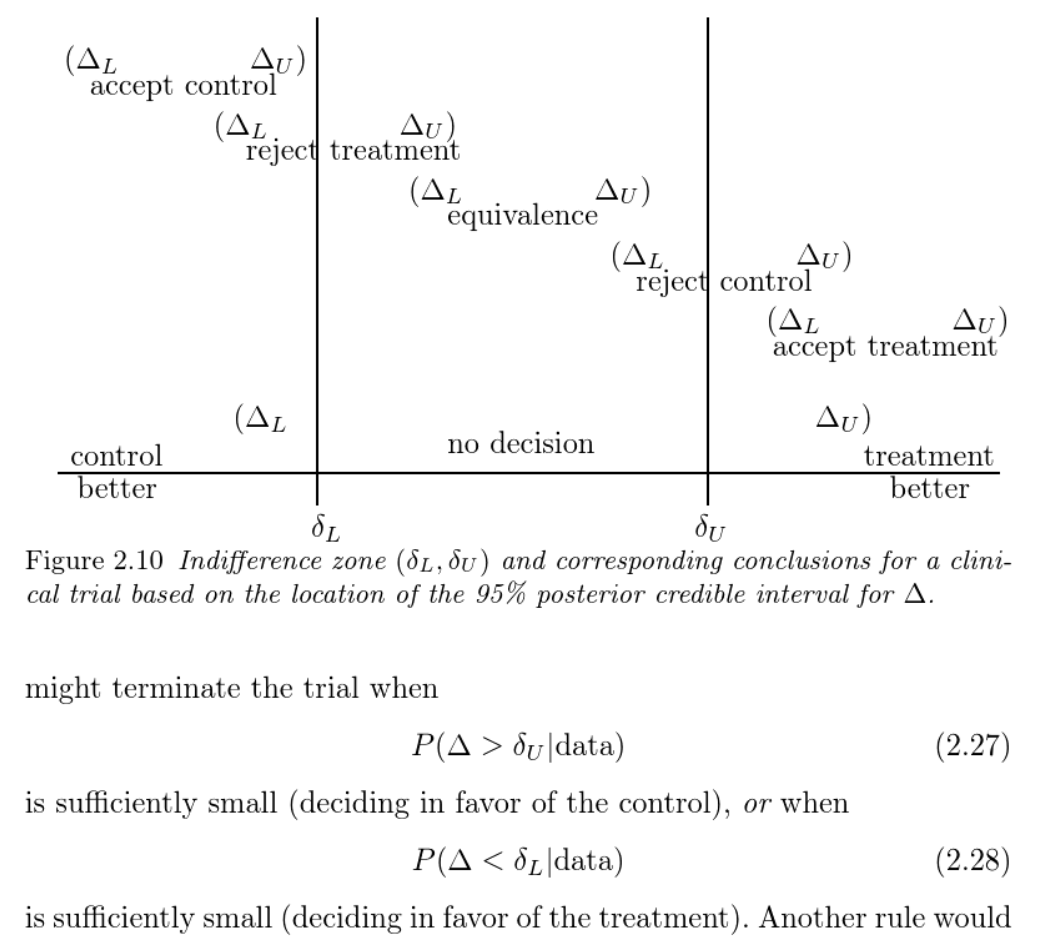
\includegraphics[width=0.75\textwidth,height=\textheight]{Figure2.10.PNG}

\begin{enumerate}
\def\labelenumi{\arabic{enumi}.}
\setcounter{enumi}{2}
\tightlist
\item
  Use of priors
\item
  Operating characteristics - Bayesian trial sample size
\end{enumerate}

Additional reading on Bayesian trial sample size

\begin{itemize}
\tightlist
\item
  \href{https://doi.org/10.1191/0962280203sm345oa}{Bayesian techniques
  for sample size determination in clinical trials: a short review}
\item
  \href{https://doi.org/10.1111/j.1467-985X.2006.00438.}{Using
  historical data for Bayesian sample size determination}
\item
  \href{https://projecteuclid.org/journals/statistical-science/volume-15/issue-2/Clinical-Trials-and-Sample-Size-Considerations-AnotherPerspective/10.1214/ss/1009212752.full}{Clinical
  Trials and Sample Size Considerations: Another Perspective}
\end{itemize}

Some thing interesting to read: Bayesian and type I error,
\url{https://www.fharrell.com/post/pvalprobs/}

\begin{enumerate}
\def\labelenumi{\arabic{enumi}.}
\setcounter{enumi}{4}
\tightlist
\item
  Online Bayesian Phase I and II design apps,
  \url{https://trialdesign.org/\#newsSection}
\end{enumerate}

\end{document}
